\documentclass[letterpaper,10pt]{article}

\usepackage{titling}
\usepackage{listings}
\usepackage{url}
\usepackage{setspace}
\usepackage{subfig}
\usepackage{sectsty}
\usepackage{pdfpages}
\usepackage{colortbl}
\usepackage{multirow}
\usepackage{multicol}
\usepackage{relsize}
\usepackage{amsmath}
\usepackage{wasysym}
\usepackage{fancyvrb}
\usepackage{amssymb}
\usepackage{ifsym}
\usepackage{amsmath,amssymb,amsthm,graphicx,xspace}
\usepackage[titlenotnumbered,noend,noline]{algorithm2e}
\usepackage[compact]{titlesec}
\usepackage{XCharter}
\usepackage[T1]{fontenc}
\usepackage{tikz}
\usetikzlibrary{arrows,automata,shapes,trees,matrix,chains,scopes,positioning,calc}
\tikzstyle{block} = [rectangle, draw, fill=blue!20, 
    text width=2.5em, text centered, rounded corners, minimum height=2em]
\tikzstyle{bw} = [rectangle, draw, fill=blue!20, 
    text width=4em, text centered, rounded corners, minimum height=2em]

\definecolor{namerow}{cmyk}{.40,.40,.40,.40}
\definecolor{namecol}{cmyk}{.40,.40,.40,.40}

\let\LaTeXtitle\title
\renewcommand{\title}[1]{\LaTeXtitle{\textsf{#1}}}


\newcommand{\handout}[5]{
  \noindent
  \begin{center}
  \framebox{
    \vbox{
      \hbox to 5.78in { {\bf ECE356: Database Systems } \hfill #2 }
      \vspace{4mm}
      \hbox to 5.78in { {\Large \hfill #4  \hfill} }
      \vspace{2mm}
      \hbox to 5.78in { {\em #3 \hfill} }
    }
  }
  \end{center}
  \vspace*{4mm}
}

\newcommand{\lecture}[3]{\handout{#1}{#2}{#3}{Lecture #1}}
\newcommand{\tuple}[1]{\ensuremath{\left\langle #1 \right\rangle}\xspace}

\addtolength{\oddsidemargin}{-1.000in}
\addtolength{\evensidemargin}{-0.500in}
\addtolength{\textwidth}{2.0in}
\addtolength{\topmargin}{-1.000in}
\addtolength{\textheight}{1.75in}
\addtolength{\parskip}{\baselineskip}
\setlength{\parindent}{0in}
\renewcommand{\baselinestretch}{1.5}
\newcommand{\term}{Winter 2018}

\singlespace


\begin{document}

\lecture{ 11 --- Decomposition: Functional-Dependency Theory }{\term}{Jeff Zarnett}

\section*{Functional-Dependency Theory}

Earlier we talked about the closure of a set of functional dependencies. Recall from earlier that the closure contains all the functional dependencies that are explicitly satisfied as well as those that are logically implied. That is, if $A \rightarrow B$ and $B \rightarrow C$ then it is implied that $A \rightarrow C$ and this is true no matter how many steps are in between, because this is transitive. More formally, if the functional dependencies are $A \rightarrow B$ and $B \rightarrow C$ then we know that for two tuples $t_{1}$ and $t_{2}$ if $t_{1}[A] = t_{2}[A]$ then $t_{1}[B] = t_{2}[B]$ and $t_{1}[C] = t_{2}[C]$. The notation to show the closure of a set $F$ of functional dependencies is $F^{+}$ as previously discussed.

It is unlikely, however, that we want to compute $F^{+}$ from the definition of functional dependencies; if $F$ is large there are many rules and many implied rules and we have to construct every logically implied element of $F^{+}$ from first principles. Instead, we would like to use \textit{axioms}, handy rules of inference, that allow us to reason about the dependencies in a simpler way. The first three axions are simple enough and are called \textit{Armstrong's Axioms}, named after the person who came up with them~\cite{dsc}:

\begin{itemize}
	\item \textbf{Reflexivity}: If $\alpha$ is a set of attributes and $\beta$ is contained within $\alpha$, then $\alpha \rightarrow \beta$ holds.
	\item \textbf{Augmentation}: If $\alpha \rightarrow \beta$ holds and $\gamma$ is a set of attributes, then $\gamma\alpha \rightarrow \gamma\beta$ holds.
	\item \textbf{Transitivity}: If $\alpha \rightarrow \beta$ holds and $\beta \rightarrow \gamma$ holds, then $\alpha \rightarrow \gamma$ holds.
\end{itemize}

These axioms are considered both sound and complete, because they do not produce any errors and they allow generation of $F^{+}$ given $F$. There are proofs of these properties, but we prefer to omit those and just focus on using them. This is a minimal set, though, and there are some rules that we can derive some more from Armstrong's rules that would be convenient shortcuts~\cite{dsc}:

\begin{itemize}
	\item \textbf{Union}: If $\alpha \rightarrow \beta$ holds and $\alpha \rightarrow \gamma$ holds, then $\alpha \rightarrow \beta\gamma$ holds.
	\item \textbf{Decomposition}: If $\alpha \rightarrow \beta\gamma$ holds, then  $\alpha \rightarrow \beta$ holds and $\alpha \rightarrow \gamma$ holds (reverse of previous rule).
	\item \textbf{Pseudotransitivity}: If $\alpha \rightarrow \beta$ holds and $\gamma\beta \rightarrow \delta$ holds, then $\alpha\gamma \rightarrow \delta$ holds.
\end{itemize}

We'll work on the example in the textbook(\cite{dsc}) which says that the relation $r$ has the attributes $(A, B, C, G, H, I)$ and the functional dependencies are: (1) $A \rightarrow B$, (2) $A \rightarrow C$, (3) $CG \rightarrow H$, (4) $CH \rightarrow I$, (5) $B \rightarrow H$.

Based on the rules that we have, what logically implied functional dependencies can we observe? 

There are three~\cite{dsc}:
\begin{itemize}
	\item $A \rightarrow H$ which is found by transitivity ($A \rightarrow B$ and $B \rightarrow A$).
	\item $CG \rightarrow HI$ which is found by the union rule ($CG \rightarrow H$ and $CG \rightarrow I$).
	\item $AG \rightarrow I$ which is found by pseudotransitivity ($A \rightarrow C$ and $CG \rightarrow I$). 
\end{itemize}

The full algorithm for building up the closure just uses Armstrong's rules and is as below. The algorithm terminates when there is nothing left to add, which is certain to happen because the worst case scenario is that everything is functionally dependent on everything else which would mean if there are $n$ attributes, there are $2^{n} \times 2^{n}$ possible functional dependencies. Now, the algorithm~\cite{dsc}:

\begin{enumerate}
	\item The initial condition is that $F^{+}$ begins as $F$.
	\item For each functional dependency $f$ in F+ $F^{+}$:
	\begin{enumerate}
		\item apply the transitivity rule to $f$ and add it to $F^{+}$
		\item apply the augmentation rule to $f$ and add it to $F^{+}$
	\end{enumerate}
	\item For each pair of functional dependencies $f_{1}$ and $f_{2}$, if they can be combined using transitivity, add the newly created combination to $F^{+}$.
	\item If anything was added in steps 2 or 3, go back to step 2; otherwise the algorithm terminates.
\end{enumerate}

\paragraph{Closure of Attribute Sets.} Suppose we have some attribute(s) $\alpha$ and we wish to determine if it is a superkey. The strategy we will use requires us to compute the set of attributes that are \textit{functionally determined} by $\alpha$. An attribute $B$ is functionally determined by $\alpha$ if $\alpha \rightarrow B$. Then the  simple algorithm requires us to compute $F^{+}$ as above and then take all functional dependencies where $\alpha$ is the left hand side and the union of the right hand side of all dependencies, but this is difficult and expensive because $F^{+}$ may be large. Instead, a more efficient algorithm follows~\cite{dsc}.

\begin{enumerate}
	\item The initial condition is that $\alpha^{+}$ begins as $\alpha$.
	\item For each functional dependency $\beta \rightarrow \gamma$ in $F$,
		if $\beta$ is contained in $\alpha^{+}$, then $\gamma$ is added to $\alpha^{+}$
	\item If anything was added in step 2, repeat step 2; if nothing was added, the algorithm terminates.
\end{enumerate}

Much like computing the closure of $F$, here we compute the closure of $\alpha$. 

Going back to the earlier example with the five functional dependencies, we would like to evaluate something to see if it is a superkey. Given the rules, is $A$ a superkey? Let's go through the steps. 

The initial condition is that $A$ is in $\alpha^{+}$ (the result). Based on the rules, we can look at the rule $A \rightarrow B$ and see that we can add to the result $B$, which is now $AB$. The next rule that says $A \rightarrow C$ allows us to add $C$ to the result so $ABC$. The rules that require $CG$ on the left hand side cannot be added, at least not yet, because $CG$ does not appear in the result ($C$ does, but not $G$). We can look at the rule for $B \rightarrow H$ and add $H$ to the result meaning the result is $ABCH$. This is not the full set ($ABCGHI$) and therefore we conclude that $A$ is not a superkey.

This procedure can be repeated for any individual attribute and we will quickly find that no single attribute is a superkey for this relation. This is perhaps somewhat obvious from our list of functional dependencies. If we look carefully at them we can notice that neither $A$ nor $G$ ever appears on the right hand side of any of the functional dependencies, but all the other attributes do. That gives us a hint that a superkey might be $AG$, and that assumption can of course be tested by following the rules as above.

If our candidate is $AG$ as suggested, we start off by saying the result is $AG$. Then  iterating through the functional dependencies: the first rule of $A \rightarrow B$ means we can add $B$ to get $ABG$. The next rule of $A \rightarrow C$ lets us make the result $ABCG$. The dependency $CG \rightarrow H$ allows us to add $H$ and get $ABCGH$, and the dependency $CG \rightarrow I$ means the result is $ABCGHI$ which encompasses all attributes and we can terminate the algorithm here; our guess based on the hints was a good one.

There are three ways we can use this attribute closure algorithm~\cite{dsc}:
\begin{itemize}
	\item As above, to test if $\alpha$ is a superkey.
	\item Check if a functional dependency holds (by determining if it is in $\alpha^{+}$.
	\item As another way to compute $F^{+}$; we just compute the $\alpha^{+}$ for each $\alpha$ and then combine them. 
\end{itemize}

\subsection*{Canonical Cover}
Suppose we have a set of functional dependencies $F$ on a relation. Whenever a user wants to update the data inside this relation, the database system must check that all functional dependencies in $F$ are still satisfied (i.e., no key constraints or other rules are broken)~\cite{dsc}. It is worth noting that in real life the rules are only enforced if you actually tell the database about them. If an update or insertion is inconsistent with the established rules, it is not permitted to happen.

Rather than checking every single functional dependency exactly as it is written, which may have some redundancy, we would like to simplify the set to a minimal number of rules that has the same closure. For example, if the rules say $A \rightarrow B$ and $B \rightarrow C$ and $A \rightarrow C$ we can immediately identify that there is redundancy and we could remove the rule $A \rightarrow C$ and still get the same closure, because that rule is implied and need not be checked separately.

You could argue that this sort of thing should not be necessary: designers should not introduce redundant rules and if they do it is their own fault. That is nice, but we don't live in a perfect world. Database designers who sit down and work out functional dependencies in advance and draw diagrams and plan ahead will probably have few redundant rules. But that's not what happens a lot of the tine, either the system is designed well and then grows to have duplicate rules over time, or, very commonly, people just create some tables without thinking about it much and ``we'll fix it later if we have to'' is the approach. But it's hard to fix later, and in the meantime, the database has done a lot of unnecessary work...

Formally speaking, an attribute of a functional dependency is \textit{extraneous} (unnecessary) under the following two scenarios~\cite{dsc}:
\begin{itemize}
	\item $A$ is extraneous in $\alpha$ if $A$ is in $\alpha$ and $F$ logically implies $(F - (\alpha \rightarrow \beta)) \cup ((\alpha - A) \rightarrow \beta))$.
	\item $A$ is extraneous in $\beta$ if $A$ is in $\beta$ and the set of functional dependencies $(F - (\alpha \rightarrow \beta)) \cup (\alpha \rightarrow (\beta - A))$ logically implies $F$.
\end{itemize}

The first scenario is about removing a redundant attribute $A$ from the left hand side of an implication; the second is about removing it from the right hand side. An example of the first is if our rules say $AB \rightarrow C$ and $A \rightarrow C$, then we could remove $B$ from the left hand side. For the other scenario, if $AB \rightarrow CD$ and $A \rightarrow C$ are the functional dependencies, then $C$ is extraneous in the right hand side~\cite{dsc}.

To check if $A$ is extraneous on the right hand side, the routine is fairly simple; remove $A$ from the right hand side ($\beta$) from the rule that it is in (e.g., if the rule is $D \rightarrow AB$, replace it with $D \rightarrow B$) and then compute the canonical cover of $\alpha$ (in this example, $D$). If the canonical cover included $A$, then $A$ was extraneous in $\beta$.

To check if $A$ is extraneous on the left hand side, the idea is pretty much the same: remove $A$ from the left hand side ($\alpha$) and check if this reduced set still functionally determines $\beta$. So if the rule is $DF \rightarrow GH$, remove $F$ and we are left with the uncertain rule $D \rightarrow GH$, which we need to test to be sure. We compute the closure of $D$ without this modified rule and see if it includes $GH$ (actually, all attributes in $\beta$). If it does, then $F$ was extraneous in the left hand side.

The canonical cover for $F$ is denoted $F_{c}$ and it is a minimal representation of $F$. It requires two rules: (1) no functional dependency in $F_{c}$ has an extraneous attribute, and (2) the left side of each functional dependency is unique. The second rule means we can't have two rules that say $A \rightarrow B$ and $A \rightarrow C$ respectively; we must combine them in one single rule $A \rightarrow BC$. By making the minimal set, it makes it easier to test if the functional dependencies are satisfied.

Let's do an example from~\cite{dsc}: The schema is simple $(A, B, C)$ and our functional dependencies are ($A \rightarrow BC, B \rightarrow C, A \rightarrow B, AB \rightarrow C$). Well, anyway, it is simple enough, we can use the union rule to combine the rule $A \rightarrow BC$ and $A \rightarrow B$ (pretty obvious). And then we can remove extraneous attributes to get this down to $A \rightarrow B$ and $B \rightarrow C$. This is slightly redundant and we can figure out by transitivity that $A \rightarrow BC$. These rules are pretty easy to test and we prefer to test these two versus the original four. This is a pretty terrible schema, actually, because there are way too many dependencies and only three attributes. 

Let's try instead a different one from~\cite{fds}: our schema has more attributes and the functional dependencies are ($B \rightarrow A, D \rightarrow A, AB \rightarrow D$). In this case, all the left hand sides are different, so we can't combine any that way. The right hand sides are all single attributes so we don't need to look for extraneous attributes there. But we should look at the left hand side. The only one that is not minimal there is the functional dependency $AB \rightarrow D$ and we would like to know if we can eliminate $A$ or $B$ from the left side. Looking at the rule that says $B \rightarrow A$ we can probably reason pretty well that if $B \rightarrow A$ then $B \rightarrow AB$  (which you can also reason as adding $B$ to both sides of the rule $B \rightarrow A$ becomes $BB \rightarrow AB$ and $BB$ is just $B$). So we can replace the one double-left-side rule with $B \rightarrow D$. Then we have a set that is equivalent: ($B \rightarrow A, D \rightarrow A, B \rightarrow D$). There is some redundancy here, though, and we could find out that $B \rightarrow A$ can be eliminated, leaving us with ($B \rightarrow D, D \rightarrow A$).

Because canonical cover is about finding a minimal equivalent set, it is not necessarily that there is only one correct answer. If there is redundancy, we may need to delete one of two attributes (but not both). Let's go back to the example from earlier with the three attributes. Our functional dependencies are still ($A \rightarrow BC, B \rightarrow C, A \rightarrow B, AB \rightarrow C$). If we test $A \rightarrow BC$ we will find that both $B$ and $C$ are extraneous. This is normally not an issue, because we just test one of the two, and if it is redundant, we delete it and move on to testing other attributes in the modified set. But one person might choose to delete $B$ and another person might choose to delete $C$. Neither choice is wrong, but they will produce two different canonical cover sets, both of which are equally correct. The more functional dependencies there are with redundancy to be eliminated, the more possible correct answers there are. 


\subsection*{Lossless Decomposition}

Decomposition is breaking up a relation into two or more smaller ones. The motivations for doing so are something we will come back to later on, but for the moment, just assume there are good reasons. A decomposition is \textit{lossless} if no information is lost by splitting a relation $r$ into smaller relations $r_{1}$ and $r_{2}$; if information is lost it is called \textit{lossy} (and that is undesirable). The more precise definition of this is specified in relational algebra as $\Pi_{R_{1}}(r) \bowtie \Pi_{R_{2}}(r) = r$ (or in SQL, the natural join of the two tables with all attributes)~\cite{dsc}. 

How can we tell if a join is lossless or lossy? You may have guessed just from the placement in the topics covered that this has something to do with the functional dependencies (meta gaming the lectures?) and that would be correct. If the decomposition is lossless then every functional dependency $f$ in $F$ holds in spite of the fact that the relation is split. But we can't really cheat and just ``forget'' to put in the functional dependencies to make it work, now can we?

Thinking carefully about the way the decomposition must work, there needs to be some attribute or attributes that link together the two tables. This does mean some data is duplicated. One relation needs to have some way of referencing another, something like an address that references a person meaning the address relation contains the identifier of the person. 

The formal definition for a lossless decomposition says that one of the following must hold on the two relations: $R_{1} \cap R_{2} \rightarrow R_{1}$ or  $R_{1} \cap R_{2} \rightarrow R_{2}$. That is to say, the intersection of the two relations most be sufficient to uniquely identify one of the two of them. 

If we have employee with \textit{id, name, street, city, province, postalcode} and we tried to split it into $r_{1}$ as \textit{id, name}, and $r_{2}$ as \textit{name, street, city, province, postcode}. Is this going to work? The intersection of these two is \textit{name} and this is not a superkey for either $r_{1}$ or $r_{2}$ because names are not unique.

There is a formal way for testing that dependencies have been preserved. There is a computationally expensive algorithm outlined in the textbook, as well as one that is premised on the idea that if each functional dependency $f$ can be tested on one relation only, then just test it on that relation and we're done. Unfortunately that last assumption is not necessarily true; it could happen that a functional dependency is across tables...

Our solution is then a modified algorithm that does not require us to compute the closure of $F$. The algorithm is as follows, executed for each functional dependency $\alpha \rightarrow \beta$ ~\cite{dsc}:


\begin{enumerate}
	\item $result$ = $\alpha$
	\item for reach relation $R_{i}$ in the decomposition
	\begin{enumerate}
		\item $result = result \cup (  (result \cap R_{i})^{+} \cap R_{i} )$
	    \item if $result$ did not change at all, break out of the for loop
	    \end{enumerate}
\end{enumerate}

If $result$ contains all attributes in $\beta$, then the dependency is preserved. And this must hold for all dependencies $\alpha \rightarrow \beta$.

Which is explained in two key ideas as follows. The first idea is testing if each dependency $\alpha \rightarrow \beta$ is satisfied in $F'$, where $F'$ is the union of the \textit{restrictions} of $F$. That is, when we take the part of $F$ that can be applied to a relation $R_{i}$ we get $F_{i}$ and $F'$ is the union of all $F_{i}$s. We compute the closure of $\alpha$ under $F'$ to see if that includes $\beta$. The second idea is to use a modified version of the attribute closure algorithm to compute closure under $F'$ without actually computing $F'$ which would be expensive. For full details, see~\cite{dsc}, but keep in mind this is polynomial time rather than exponential time like computing $F^{+}$ would be.

\subsection*{Algorithms for Decomposition}

We have looked at very simple schemas (and probably will continue to look at very simple ones in this course). For those it is not too difficult to see how to get the schema into BCNF or 3NF or design it that way in the first place. But if we need to take a schema and decompose it, for a sufficiently complex schema, there are some algorithms that make this process consistent.

\paragraph{BCNF.}To decompose to BCNF, the algorithm is as follows~\cite{dsc}. The initial state is the relations that we have, and we also need to then compute $F^{+}$. Then the steps are:

\begin{center}
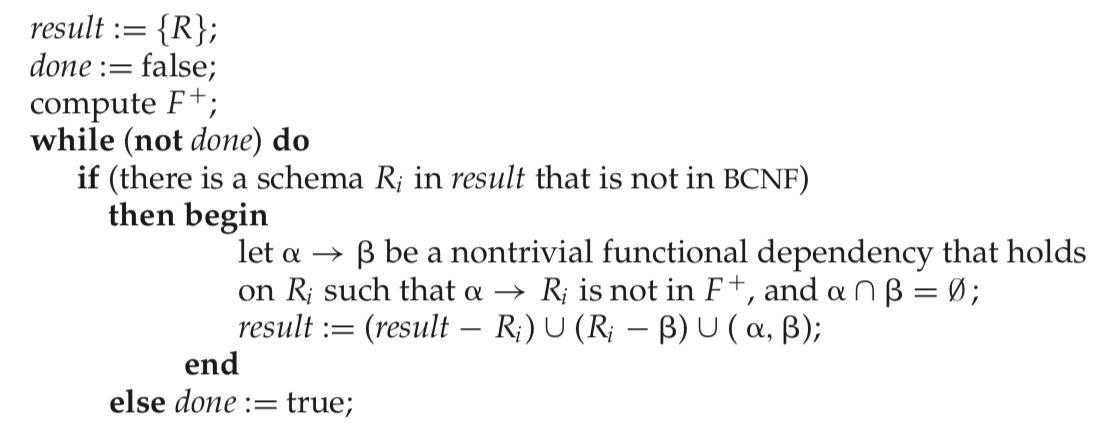
\includegraphics[width=0.7 \textwidth]{images/bcnf-algorithm}\\
BCNF Decomposition algorithm in pseudocode~\cite{dsc}
\end{center}

The algorithm produces relations in BCNF and a lossless decomposition. This is because when we replace a schema $R_{i}$ with $(R_{i} - \beta)$ and $(\alpha, \beta)$ then the intersection of these two relations is $\alpha$.

\paragraph{3NF.} If instead we wanted to put things in 3NF, it is a somewhat more complicated algorithm. It is also dependency preserving and lossless. It explicitly builds a schema for each dependency in a canonical cover, ensuring that each schema contains a candidate key. Unlike the BCNF decomposition algorithm, this builds the relations up rather than breaks them down. A formal proof of the algorithm below is in~\cite{dsc}: 

\begin{center}
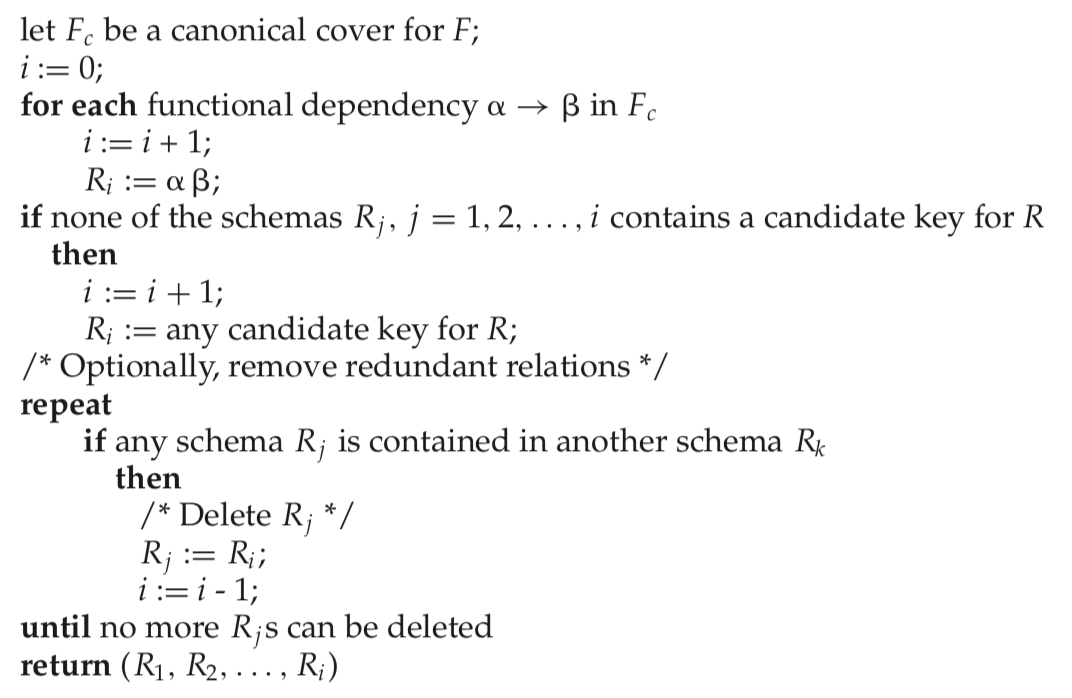
\includegraphics[width=0.7\textwidth]{images/3nf-algorithm}\\
3NF Decomposition algorithm in pseudocode~\cite{dsc}
\end{center}

\bibliographystyle{alphaurl}
\bibliography{356}


\end{document}
